\documentclass[10pt,a4paper,fleqn]{article}
\setlength{\oddsidemargin}{-1.4mm}
\setlength{\evensidemargin}{-1.4mm}
\setlength{\textwidth}{162mm}
\setlength{\topmargin}{-12mm}
\setlength{\textheight}{249mm}
\usepackage{amsmath,amssymb,bm,booktabs,array}
\usepackage{xcolor,graphicx,tikz,pgfplots}
\usepackage{url}
% Clickable, breakable URLs using pdfTeX primitives; no hyperref dependency.
\let\plainurl\url
\renewcommand{\url}[1]{\ifdefined\pdfstartlink\leavevmode\pdfstartlink attr{/Border [0 0 0]} user{/Subtype /Link /A << /S /URI /URI (\pdfescapestring{#1}) >>}\plainurl{#1}\pdfendlink\else\plainurl{#1}\fi}
\pgfplotsset{compat=1.18}
\newif\ifmarked
\markedfalse
\definecolor{revisionblue}{RGB}{18,61,130}
\newcommand{\rev}[1]{{\ifmarked\color{revisionblue}\else\color{black}\fi #1}}
\newenvironment{revision}{\begingroup\ifmarked\color{revisionblue}\else\color{black}\fi\nobreak\ignorespaces}{\par\endgroup}
\newcommand{\Eavg}{\overline{\mathcal E}_h}
\newcommand{\Cstep}{\mathcal C}
\newcommand{\Rstep}{\mathcal R}
\newcommand{\mean}[1]{\overline{#1}}
\setlength{\textfloatsep}{14pt plus 3pt minus 2pt}
\setlength{\intextsep}{14pt plus 3pt minus 2pt}
\renewcommand{\topfraction}{0.9}
\renewcommand{\textfraction}{0.08}
\renewcommand{\floatpagefraction}{0.75}
\raggedbottom
\setlength{\emergencystretch}{1em}
\pagestyle{empty}
\makeatletter
\newlabel{eq:ch}{{1}{2}{}{equation.1}{}}
\newlabel{eq:energy}{{2}{2}{}{equation.2}{}}
\newlabel{eq:structure}{{3}{2}{}{equation.3}{}}
\newlabel{eq:step}{{4}{3}{}{equation.4}{}}
\newlabel{eq:fit}{{5}{3}{}{equation.5}{}}
\newlabel{eq:ridge}{{6}{3}{}{equation.6}{}}
\newlabel{eq:candidate}{{7}{3}{}{equation.7}{}}
\newlabel{eq:discreteenergy}{{8}{3}{}{equation.8}{}}
\newlabel{eq:derivatives}{{9}{3}{}{equation.9}{}}
\newlabel{eq:massproj}{{10}{4}{}{equation.10}{}}
\newlabel{eq:accept}{{11}{4}{}{equation.11}{}}
\newlabel{eq:backtrack}{{12}{4}{}{equation.12}{}}
\newlabel{eq:descent}{{13}{4}{}{equation.13}{}}
\newlabel{eq:galerkinenergy}{{14}{5}{}{equation.14}{}}
\newlabel{eq:galerkinlaw}{{15}{5}{}{equation.15}{}}
\newlabel{eq:pidmd}{{16}{5}{}{equation.16}{}}
\newlabel{eq:adaptive}{{17}{5}{}{equation.17}{}}
\newlabel{eq:initial}{{18}{6}{}{equation.18}{}}
\newlabel{eq:errors}{{19}{7}{}{equation.19}{}}
\newlabel{eq:structureerror}{{20}{7}{}{equation.20}{}}
\newlabel{eq:violation}{{21}{7}{}{equation.21}{}}
\newlabel{eq:rectangles}{{22}{7}{}{equation.22}{}}
\newlabel{tab:accuracy}{{1}{8}{}{table.1}{}}
\newlabel{tab:epsilon}{{2}{10}{}{table.2}{}}
\newlabel{tab:mobility}{{3}{10}{}{table.3}{}}
\newlabel{tab:long}{{4}{11}{}{table.4}{}}
\newlabel{tab:timing}{{5}{12}{}{table.5}{}}
\newlabel{eq:cost}{{23}{13}{}{equation.23}{}}
\newlabel{tab:convergence}{{6}{13}{}{table.6}{}}
\newlabel{tab:teacher}{{7}{14}{}{table.7}{}}
\newlabel{tab:finer}{{8}{15}{}{table.8}{}}
\newlabel{tab:crossgrid}{{9}{15}{}{table.9}{}}
\newlabel{tab:deterministic}{{10}{15}{}{table.10}{}}
\newlabel{tab:hyper}{{11}{17}{}{table.11}{}}
\newlabel{tab:shifts}{{12}{17}{}{table.12}{}}
\newlabel{eq:fixedfilterlimit}{{24}{18}{}{equation.24}{}}
\makeatother
\begin{document}
\setcounter{figure}{4}
\begin{figure}[htbp]\centering
\begin{tikzpicture}
\begin{axis}[width=.78\textwidth,height=5.4cm,grid=major,grid style={gray!15},tick label style={font=\footnotesize},label style={font=\small},xlabel={Mean wall time (s)},ylabel={Mean relative field error},title style={font=\small},legend style={font=\scriptsize,draw=none},legend pos=south east,xmode=log,ymode=log]
\addplot[thick,solid,mark=*,mark size=2pt,mark options={solid},blue!65!black] coordinates {(0.016564772,0.0712055693) (0.094260512,0.0146881026) (0.191263852,0.00753412868) (0.374567168,0.00381698525) (1.57047379,0.000925458316)};
\addlegendentry{Coarse}
\addplot[thick,dashed,mark=square*,mark size=2pt,mark options={solid},orange!85!black] coordinates {(0.013084796,1.33890907e-07) (0.024184356,8.54149664e-09) (0.0487615,5.45551361e-10)};
\addlegendentry{ETDRK4}
\addplot[thick,dashdotted,mark=triangle*,mark size=2pt,mark options={solid},teal!80!black] coordinates {(0.035061276,0.0597951629) (0.134702308,0.0176597485) (0.460871796,0.00536972528)};
\addlegendentry{Adaptive coarse}
\addplot[thick,densely dotted,mark=diamond*,mark size=2pt,mark options={solid},purple] coordinates {(0.035615104,1.94868754e-08) (0.035847896,1.94868754e-08) (0.035473944,1.94868754e-08)};
\addlegendentry{Adaptive ETD}
\addplot[thick,dashdotdotted,mark=pentagon*,mark size=2pt,mark options={solid},black] coordinates {(0.141708088,0.00773550492)};
\addlegendentry{Residual}
\addplot[thick,loosely dashed,mark=x,mark size=2pt,mark options={solid},red!70!black] coordinates {(0.00874757999,0.0738642488)};
\addlegendentry{piDMD}
\end{axis}
\end{tikzpicture}
\rev{\caption{\rev{Achieved relative field error versus online wall time over $T=0.0035$ on the legacy $64^2$ spatial system, with $\epsilon=0.020$, $M=1$ and a refined ETDRK4 reference. Errors average five initial fields; times average five repetitions per field. Sample standard deviations are in Table~\ref{tab:timing}; no uncertainty bands are implied. Uncorrected propagation uses blue solid circles; fixed ETDRK4, orange dashed squares; adaptive stabilized propagation, teal dash-dot triangles; adaptive ETDRK4, purple dotted diamonds; the residual surrogate, a black pentagon; and piDMD, a red cross. The last two methods each contribute one configuration. The three adaptive ETDRK4 settings have identical errors because the maximum step is reached. Residual timings include correction and acceptance work; fixed ETDRK4 coefficients are warmed before timing.}}\label{fig:cost}}
\end{figure}
\clearpage
\end{document}
